\documentclass[12pt]{article}
%\nonstopmode %Debug: Evita erros de packages nao inclusos

%Codificacao do arquivo e acentos
\usepackage[T1]{fontenc}
\usepackage[utf8]{inputenc}
\usepackage[brazilian]{babel}

%Fonte e formatacao de paragrafos
\usepackage{times}
\usepackage{indentfirst}
\usepackage{setspace}

%Pacote para carregar imagens
\usepackage{graphicx}

%Margens e formatacao de pagina
\usepackage{geometry}
\geometry{a4paper, total={210mm,297mm}, left=30mm, right=20mm, top=30mm, bottom=20mm}

%Numero paginas
\usepackage{lastpage}

%Incluir outros pdfs
\usepackage{pdfpages}

%Numeros romanos para Tabelas
\renewcommand{\thetable}{\Roman{table}}

\begin{document}

%Folha de rosto
	\begin{titlepage}
		\begin{center}
			{
				\fontsize{16pt}{\baselineskip}\fontfamily{\familydefault}\selectfont 
				UNIVERSIDADE DO ESTADO DE SANTA CATARINA \\
				CENTRO DE CIÊNCIAS TECNOLÓGICAS - CCT \\
				ENGENHARIA MECÂNICA
			}\\[6cm]
			
			{\fontsize{18pt}{\baselineskip}\fontfamily{\familydefault}\selectfont MATHEUS GIARETTA CANSIAN}\\[5.5cm]

			{\fontsize{18pt}{\baselineskip}\fontfamily{\familydefault}\selectfont \bf RELATÓRIO DE ESTÁGIO CURRICULAR}

			\vfill

			\fontsize{14pt}{\baselineskip} \fontfamily{\familydefault} \selectfont
			Joinville, SC\\[0.2cm]
			2014
		\end{center}
	\end{titlepage}
	%\pagebreak

	%Folha de rosto
	\begin{titlepage}
		\begin{center}
			{\fontsize{16pt}{\baselineskip}\fontfamily{\familydefault}\selectfont MATHEUS GIARETTA CANSIAN}\\[6cm]
			{\fontsize{18pt}{\baselineskip}\fontfamily{\familydefault}\selectfont \bf RELATÓRIO DE ESTÁGIO CURRICULAR}\\[5.5cm]
		\end{center}
		
		{
			\fontsize{14pt}{\baselineskip} \fontfamily{\familydefault} \selectfont
			
			\hspace{.45\textwidth} \begin{minipage}{.5\textwidth}
				\noindent 
				Relatório apresentado ao Curso de Engenharia Mecânica do Centro de Ciências Tecnológicas, 
				da Universidade do Estado de Santa Catarina, 
				como requisito parcial para a obtenção do grau de Bacharel em Engenharia Mecânica\\[0.6cm]
				Orientador: Fernando Hummel Lafratta\\[0.1cm]
				Supervisor: Michael Thamm
			\end{minipage}
		}
		
		\vfill
		
		\begin{center}
		{
			\fontsize{14pt}{\baselineskip} \fontfamily{\familydefault} \selectfont
			Joinville, SC\\[0.2cm]
			2014
		}
		\end{center}
	\end{titlepage}
	%\pagebreak

%Espacamento 1.5
\onehalfspacing

%Desabilita numeracao pagina
\pagenumbering{gobble}

\begin{center}
{
	{
		APROVADO EM 05/12/2014
	}\\[5cm]
	
	{	
		\begin{tabular}[t]{@{}l@{}}
			\makebox[8cm]{\dotfill}\\
		\end{tabular} \\
		Professor: Fernando Humel Lafratta \\
		Doutor em Engenharia Meânica \\
		Professor orientador
	}\\[5cm]
	
	\begin{tabular}[t]{@{}l@{}}
		\makebox[8cm]{\dotfill}\\
	\end{tabular} \\
	Professor: José Aldo Silva Lima \\
	Doutor em Engenharia Meânica \\
	Membro da banca \\
}
\end{center}
\pagebreak

%Avaliacao Universidade
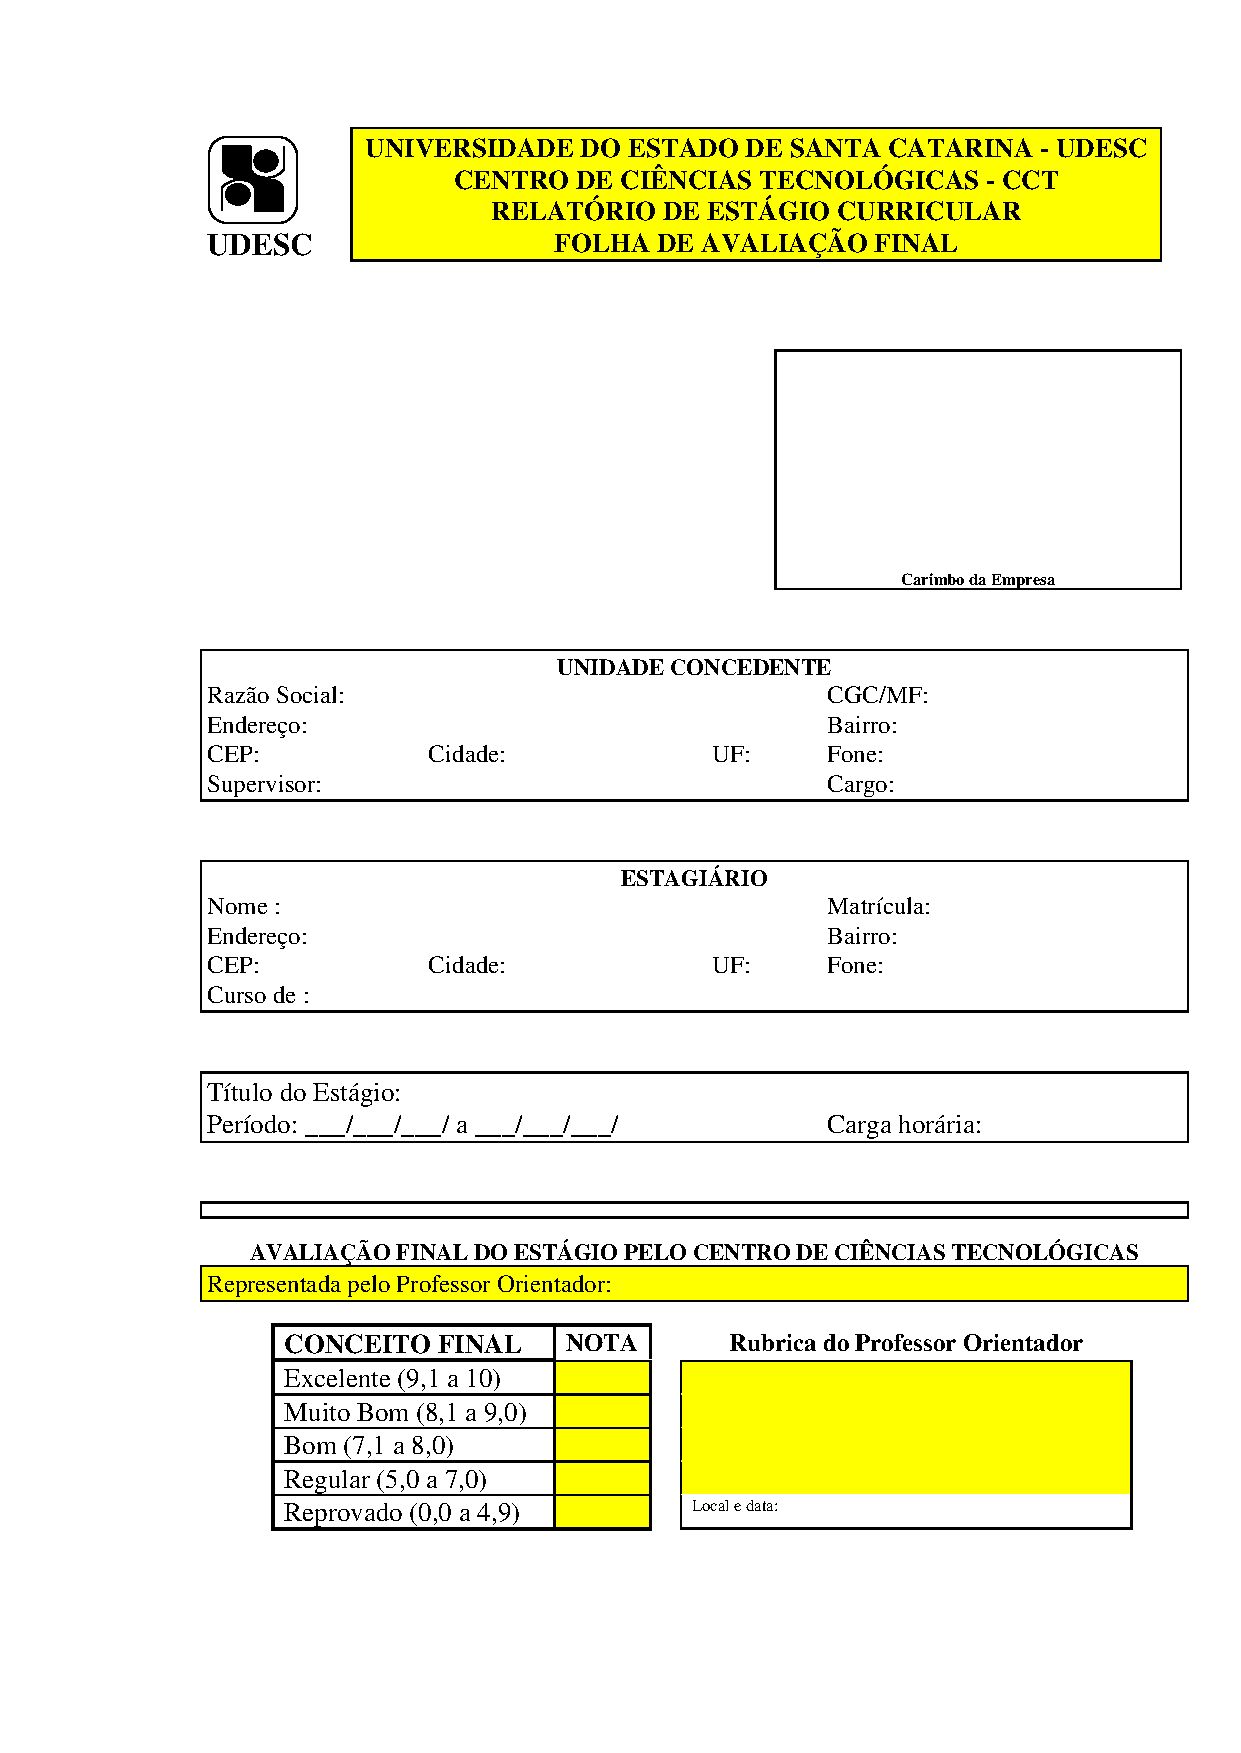
\includepdf[pages={1}]{inc/avaliacao.pdf}

%Avaliacao Empresa
\includepdf[pages={2}]{inc/avaliacao.pdf}

%Plano de estagio
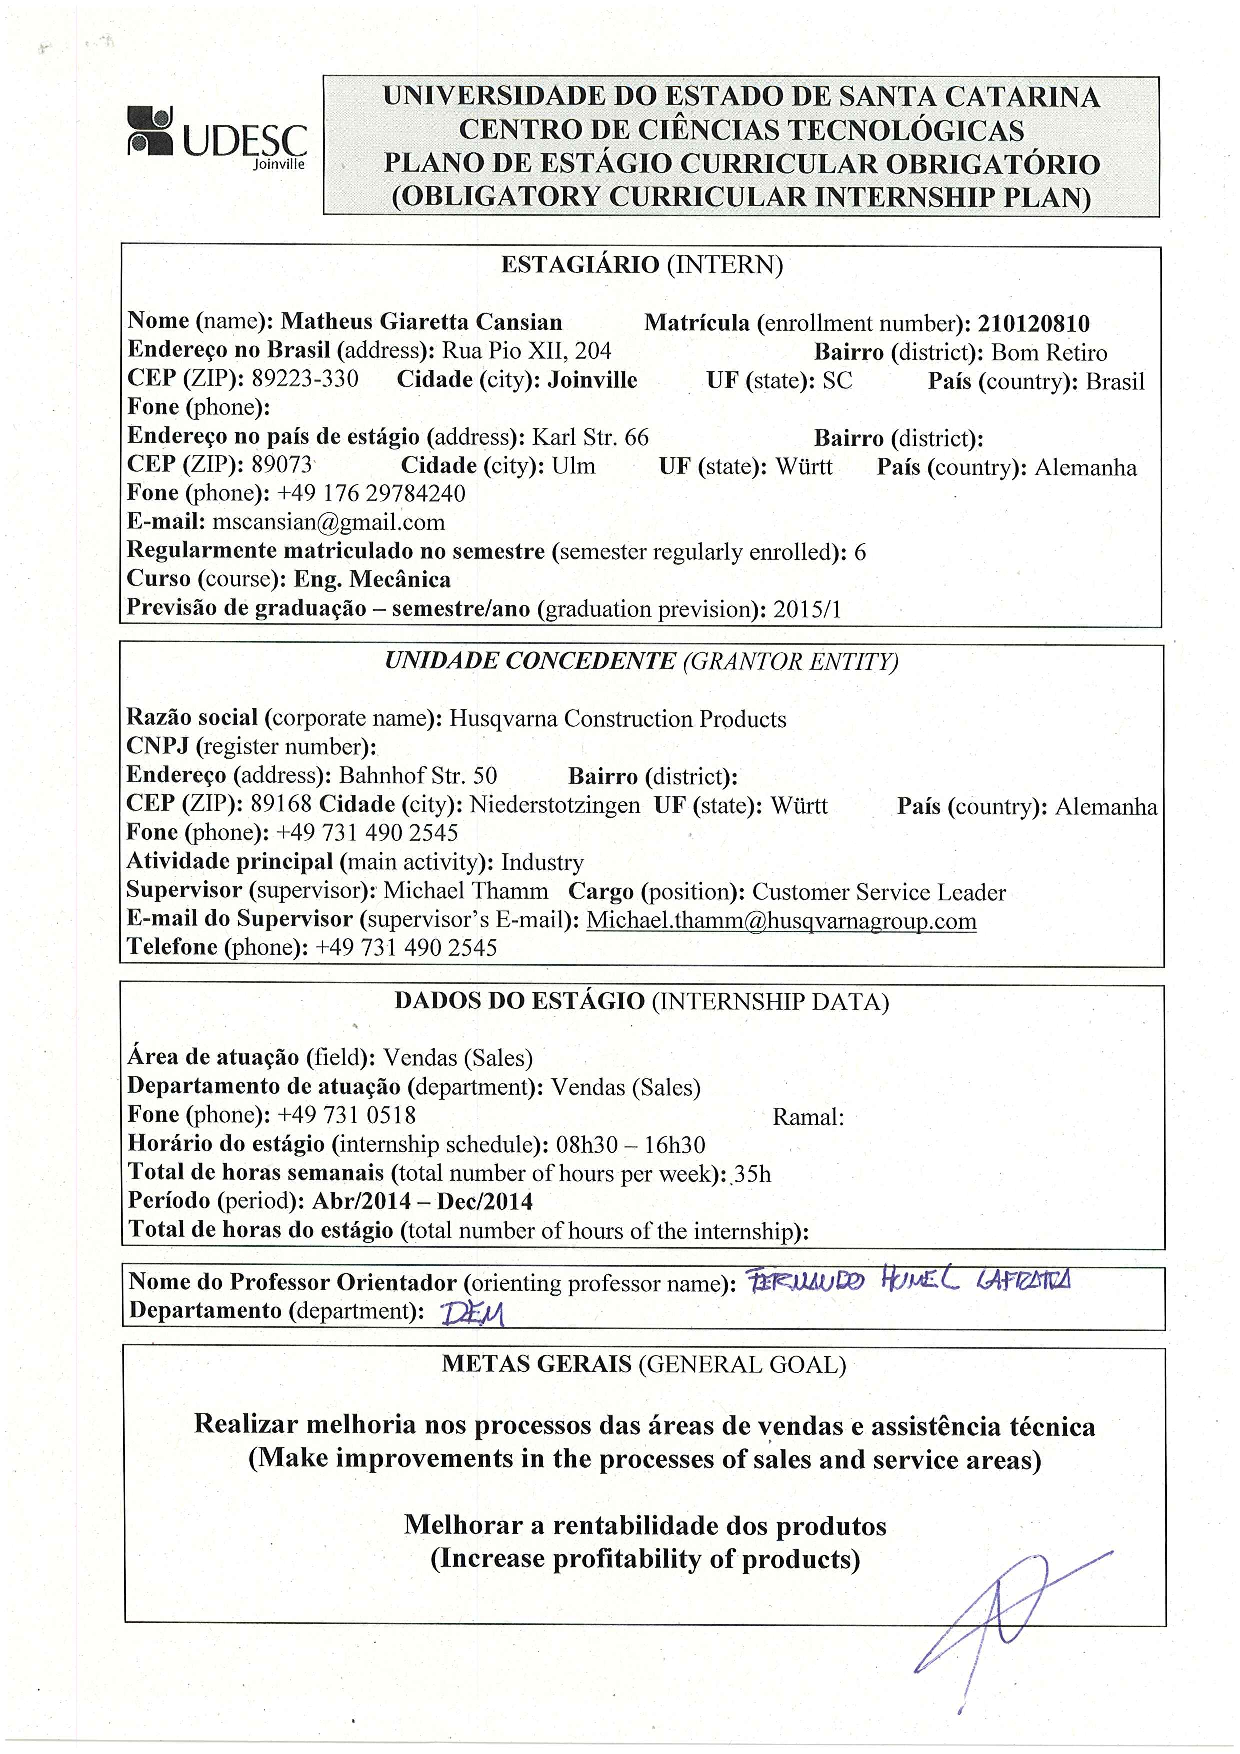
\includepdf[pages={1,2}]{inc/plano.pdf}

%Sumario
\tableofcontents
\pagebreak

%Lista de figuras
\listoffigures
\pagebreak

{
	\begin{flushleft}
	{
		\noindent
		CANSIAN, Matheus. RELATÓRIO DE ESTÁGIO CURRICULAR. 2014. \pageref{LastPage} fls. Relatório de estágio (Graduação em Engenharia Mecânica) – Universidade do Estado de Santa Catarina, Joinville, 2014. 
	}\\[2cm]
	\end{flushleft}
	
	\begin{center}
	{
		\bf RESUMO
	}\\[3cm]
	\end{center}
	
	{
		\noindent
		Apresenta algumas das atividades desenvolvidas pelo estagiário durante o período de estágio curricular do curso de Engenharia Mecânica da Universidade do Estado de Santa Catarina – UDESC, na empresa Husqvarna Construction Products, durante o período de 11 de abril de 2014 a 31 de dezembro de 2014. Os projetos realizados estão ligados à área de Vendas e Marketing do escritório de Niederstotzingen. Descreve o desenvolvimento dos projetos contidos no plano de estágio. O primeiro deles corresponde a nova política de preços para as peças de reposição e o segundo é referente à criação de um programa de manutenção de serra de parede. Apresenta breve revisão dos conceitos de administração financeira. Alguns dados foram omitidos para atender à política de confidencialidade da Husqvarna.
	}\\[1cm]

	{
		\noindent
		Palavras-chave: Vendas; Precificação; Peças de Reposição; Manutenção.
	}
}
\pagebreak

{
	\noindent
	
	\begin{flushleft}
	{
		\noindent
		CANSIAN, Matheus. REPORT OF MANDATORY INTERNSHIP. 2014. \pageref{LastPage} pages. Internship report (Major in Mechanical Engineering) – Universidade do Estado de Santa Catarina, Joinville, 2014. 
	}\\[2cm]
	\end{flushleft}
	
	\begin{center}
	{
		\bf ABSTRACT
	}\\[3cm]
	\end{center}
	
	{
		\noindent
		Presents some of the activities developed by the intern during the mandatory internship, required by Mechanical Engineering in Universidade do Estado de Santa Catarina - UDESC, in the company Husqvarna Construction Products during the period of April 11th, 2014 to December 31th, 2014. All projects developed are related to Sales and Marketing in Niederstotzingen. Describes the development of the projects written in the internship plan. The first one corresponds to new pricing policy for spare parts and the second is related to the creation of a wall saw's maintenance program. Presents a brief review of financial management concepts. Some data have been omitted to comply with Husqvarna's confidentiality policy.
	}\\[1cm]
	

	{
		\noindent
		Keywords: Sales; Pricing; Spare parts; Maintenance.
	}
}
\pagebreak

%Re-habiilita a numeracao de pagina
\pagenumbering{arabic}
\setcounter{page}{13}

\section{Introdução}

	Este relatório é resultado do estágio obrigatório realizado pelo aluno Matheus Giaretta Cansian, do curso de Bacharelado em Engenharia Mecânica, da instituição UDESC campus Joinville.
	O período no qual o estagiário atuou foi de 11 de abril de 2014 a 31 de dezembro de 2014, na empresa Husqvarna Construction Products, localizada na cidade de Niederstotzingen, Alemanha.
\pagebreak

\section{Apresentação da concedente}

	A Husqvarna é líder global em equipamentos para manejo em florestas, gramados e cuidados com o jardim. O grupo também é líder na Europa em produtos para irrigação residencial e um dos líderes mundiais em equipamentos para corte e ferramentas de diamante para a indústria da construção civil. As soluções desenvolvidas pelo grupo chegam ao mercado principalmente através de revendedores, tanto para uso doméstico quanto profissional. A Husqvarna está presente em mais de 100 países, com 14 mil funcionários e um faturamento anual de 4 bilhões do dólares.

\subsection{Marcas}

	Para atingir grupos distintos de consumidores a empresa não só utiliza a marca Husqvarna, como também outras, sendo Husqvarna, Gardena, McCulloch e Diamant Boart as principais marcas do Grupo.

\subsubsection{Husqvarna}

\begin{figure}[h!]
	\centering
	
\includegraphics[width=0.4\textwidth]{img/logo-husqvarna.png}
	\caption{Husqvarna}
\end{figure}

	Husqvarna é, há muitos anos, uma marca premium e forte em todo o mundo, representando a liderança tecnológica, desempenho profissional, alta qualidade e foco no usuário. A marca Husqvarna é responsável por aproximadamente 50\% das vendas do Grupo. Na figura \ref{fig:husq-prod} pode-se visualizar alguns dos produtos com a marca.

\begin{figure}[h!]
	\centering
	
\includegraphics[width=0.25\textwidth]{img/products/husq4.png}
	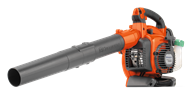
\includegraphics[width=0.25\textwidth]{img/products/husq5.png}
	
\includegraphics[width=0.25\textwidth]{img/products/husq2.png}
	\\
	
\includegraphics[width=0.25\textwidth]{img/products/husq1.png}
	
\includegraphics[width=0.25\textwidth]{img/products/husq3.png}
	
\includegraphics[width=0.25\textwidth]{img/products/husq6.png}
	\caption{Produtos Husqvarna}
	\label{fig:husq-prod}
\end{figure}

\subsubsection{Husqvarna Construction}
	Husqvarna Construction é uma subdivisão da Husqvarna que produz produtos voltados para a construção civil. Na prática não existe nenhuma diferenciação de marca, todos os produtos utilizam o nome Husqvarna. A única mudança se encontra na apresentação do portfólio e na estrutura interna do grupo. Os produtos de construção são divididos nas seguintes categorias: Furadeiras profissionais; Serras circulares; Serras de mesa e produtos para azulejo; Serras de parede; Preparação de superfície; E robôs de demolição. Na figura \ref{fig:hc} pode-se ver alguns desses diferentes produtos.

\begin{figure}[h!]
	\centering
	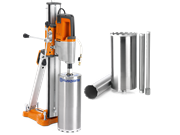
\includegraphics[width=0.3\textwidth]{img/products/cons1.png}
	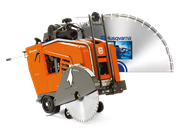
\includegraphics[width=0.3\textwidth]{img/products/cons2.png}
	
\includegraphics[width=0.3\textwidth]{img/products/cons3.png}
	\\
	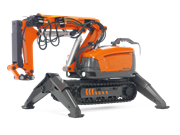
\includegraphics[width=0.3\textwidth]{img/products/cons4.png}
	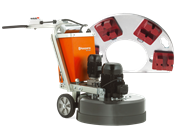
\includegraphics[width=0.3\textwidth]{img/products/cons7.png}
	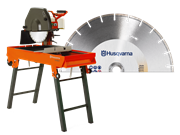
\includegraphics[width=0.3\textwidth]{img/products/cons8.png}
	\caption{Produtos Husqvarna Construction}
	\label{fig:hc}
\end{figure}


\subsubsection{Gardena}

	Gardena é a marca premium do canal varejo, líder na Europa em produtos para irrigação e ferramentas de jardim para o uso doméstico. A linha também inclui produtos movidos a bateria e representa aproximadamente 10\% das vendas do Grupo. O portfólio é dividido nas seguintes categorias: Cortadores de grama manuais; Ferramentas manuais de jardinagem; Equipamentos para irrigação; E cortadores de grama automáticos. Na figura \ref{fig:gardena-prod} pode-se visualizar um produto de cada categoria.

\begin{figure}[h!]
	\centering
	
\includegraphics[width=0.4\textwidth]{img/logo-gardena.png}
	\caption{Gardena}
\end{figure}

\begin{figure}[h!]
	\centering
	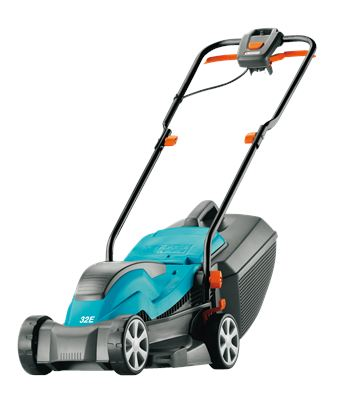
\includegraphics[width=0.25\textwidth]{img/products/gardena2.jpg}
	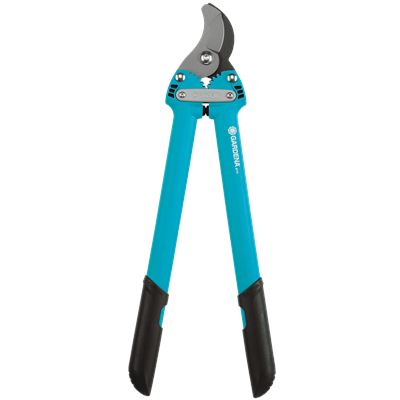
\includegraphics[width=0.25\textwidth]{img/products/gardena3.jpg}
	
\includegraphics[width=0.25\textwidth]{img/products/gardena4.jpg}
	\\	
	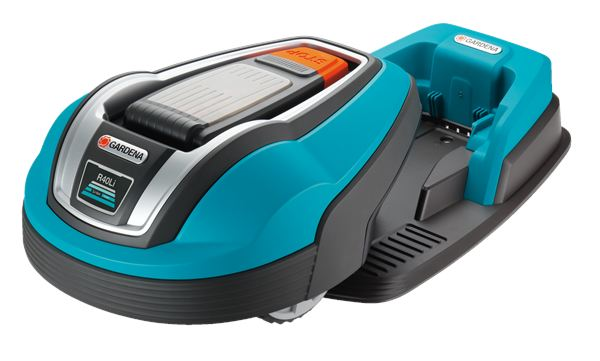
\includegraphics[width=0.25\textwidth]{img/products/gardena1.jpg}
	\caption{Produtos Gardena}
	\label{fig:gardena-prod}
\end{figure}

\subsubsection{McCulloch e Diamant Boart}

	McCulloch é uma marca premium global, incluindo produtos para manejo de florestas e jardins para consumidores exigentes do canal de varejo. Na figura \ref{fig:mc-prod} pode-se visualizar alguns dos produtos da McCulloch. 
	Diamant Boart é reconhecida como a marca líder global na indústria de pedras. A oferta de produtos inclui uma linha completa de ferramentas diamantadas para o processamento de pedra natural.

\begin{figure}[h!]
	\centering
	
\includegraphics[width=0.4\textwidth]{img/logo-mcdb.png}
	\caption{McCulloch e Diamant Boart}
\end{figure}

\begin{figure}[h!]
	\centering
	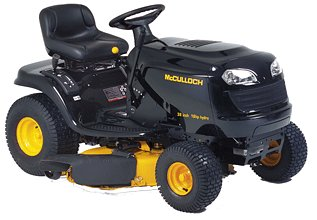
\includegraphics[width=0.3\textwidth]{img/products/mc1.jpg}
	
\includegraphics[width=0.3\textwidth]{img/products/mc2.jpg}
	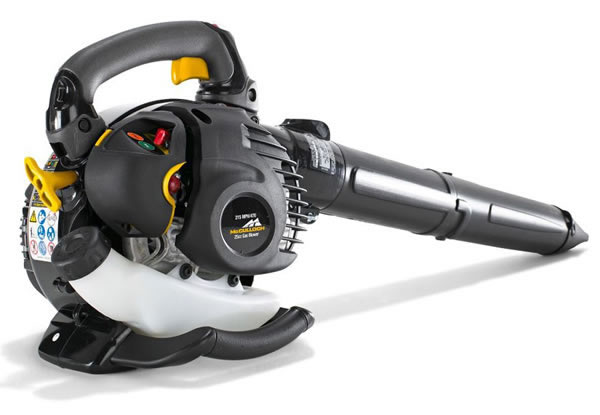
\includegraphics[width=0.3\textwidth]{img/products/mc3.jpg}
	\caption{Produtos McCulloch}
	\label{fig:mc-prod}
\end{figure}

\subsection{Visão}
	``Vislumbramos um mundo onde as pessoas possam desfrutar de jardins, parques e florestas bem cuidados e experimentar estradas e edifícios refinados.''

\subsection{Missão}
	``Fornecemos soluções e produtos inovadores e de qualidade para tornar mais fácil o cuidado de jardins, parques e florestas, bem como as atividades do setor de construção, para profissionais e consumidores ao redor do mundo.''

%Construction é responsavel por 10\% do faturamento do grupo
	
\subsection{História}
	Em 1620 foi fundada a empresa “Jönköping Rifle Factory”, por decreto do rei da Suécia e durante os primeiros anos essa fábrica produziu cerca de 1.500 tubos de mosquete anualmente. A assinatura do produto inspirou o logotipo clássico “mira de mosquete” que, apesar de atualizado, é usado ainda hoje.
	Quando a Suécia começou a aumentar seu exército em 1689, nasceu oficialmente a fábrica da Husqvarna para perfuração e moagem de tubos de mosquete, a 7 km de Jönköping nas cachoeiras Huskvarna (escrita antiga de Husqvarna) - lugar no qual agora localiza-se o moderno complexo da fábrica da Husqvarna.

	O contrato de produção de rifles Husqvarna para a Coroa chegou ao fim e a empresa começou a procurar maneiras de diversificar. Isto tornou-se o início de um período muito inovador e ambicioso, que resultou em ampla gama de novos produtos, tais como: máquinas de costura (1872), armas de caça (1877), fogões de madeira (1884), máquinas de moer (1890), a primeira máquina de escrever sueco (1895), bicicletas (1896), motocicletas (1903) e fogões a gás (1912).

	Em 1918 a Husqvarna adquiriu “Norrahammars Bruk”, adicionando dois novos produtos ao seu portfólio: caldeiras e cortadores de grama manuais. Em 1919, a empresa começou a fabricar seus próprios motores.

	Em 1972 o nome da empresa foi oficialmente abreviado para simplesmente “Husqvarna”, que foi implementado juntamente com o logotipo atual.

%\subsection{Principais produtos}
%Os produtos na área de construção se dividem nas categorias que serão apresetadas a seguir.

\subsection{Mercado de construção civil na Alemanha}

	O mercado de construção civil na Alemanha é marcado pelo alto custo da mão de obra. Por este motivo, máquinas que agilizam a construção são muito funcionais e demandadas. No portfólio da empresa existem máquinas como uma serra de parede que custa mais de 150 mil reais. Este custo se justifica, pois um equipamento deste porte agiliza o trabalho e faz com que uma obra seja feita em tempo padrão, com mão de obra menor. Existem outros produtos como uma furadeira automática que aumenta a produtividade em 2 vezes: o operador monta a máquina e realiza um furo e no tempo em que esta está operando, ele pode montar uma segunda máquina. Quando a segunda furadeira esta pronta, a primeira já terá terminado o furo.

	Outra peculiaridade das construções alemãs é que os pré-moldados são muito utilizados. Isso diminui o tempo necessário para executar uma obra.

\subsection{Tipos de clientes}

	O mercado da Husqvarna é composto por dois perfis de clientes com características distintas. O primeiro deles é chamado internamente de OTS (On-the-shelf) e corresponde aos revendedores de máquinas, que são responsáveis por distribuir essas máquinas aos profissionais de pequeno porte e outros consumidores interessados em produtos de construção. Para este grupo, a Husqvarna fornece equipamentos mais genéricos e menos profissionais, sendo as serras circulares, as serras de mesa e as furadeiras mais simples os principais produtos consumidos. A decisão de compra é caracterizada por maior foco no aspecto marketing e menos em aspectos técnicos.

\begin{figure}[h!]
	\centering
	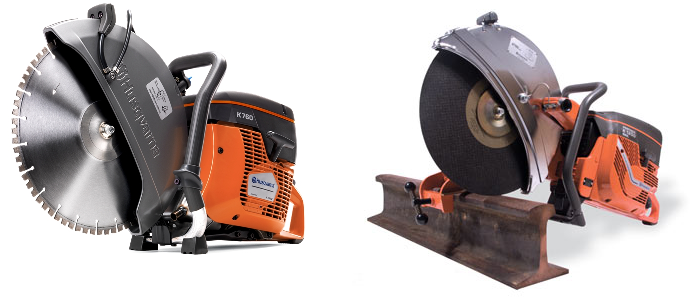
\includegraphics[width=0.9\textwidth]{img/k760-vs-k1260rail.png}
	\caption{K760 e K1260 RAIL}
	\label{fig:k700vsk1260}
\end{figure}

\begin{figure}[h!]
	\centering
	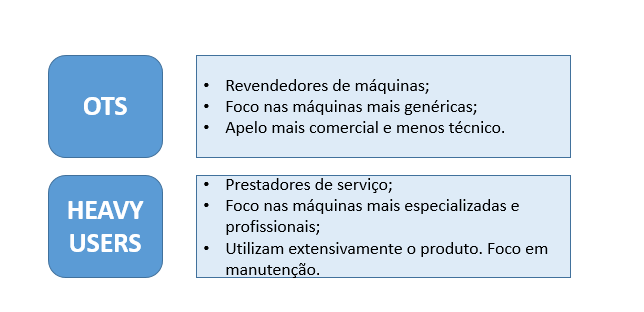
\includegraphics[width=0.9\textwidth]{img/clientes-pt.png}
	\caption{Tipos de clientes}
	\label{fig:tipo-clientes}
\end{figure}

	O segundo grupo é conhecido como "heavy users" e corresponde aos prestadores de serviço de médio e grande porte. Este público necessita de máquinas mais profissionais e robustas e os principais produtos consumidos são as serras mais pesadas, serras de chão, robôs de demolição e serras de parede. A decisão de compra, nesse caso, é mais focada nos aspectos técnicos do produto (custo de manutenção, potência, eficiência) e isto exige da Husqvarna um portfólio com soluções extremamente especializadas, que realizam determinados serviços com a maior eficiência possível. Os heavy users realizam serviços diversos de construção e em geral, utilizam o maquinário no dia-a-dia. A sofisticação dessta linha de produtos requer suporte e manutenção mais cuidadosos, pois alguns produtos tendem a ter mais de 400 horas de uso ao ano. 
	
	Na figura \ref{fig:k700vsk1260}, pode-se visualizar a diferença entre uma máquina genérica (à esquerda) e uma máquina especializada em cortar de trilhos de trem. A máquina especializada, apesar de executar apenas um tipo de serviço, o faz com melhor eficiência. Na figura \ref{fig:tipo-clientes} pode-se visualizar as principais características de cada grupo de clientes.
	


%\subsection{Estrutura administrativa}

%\begin{figure}[!ht]
%	\centering
%	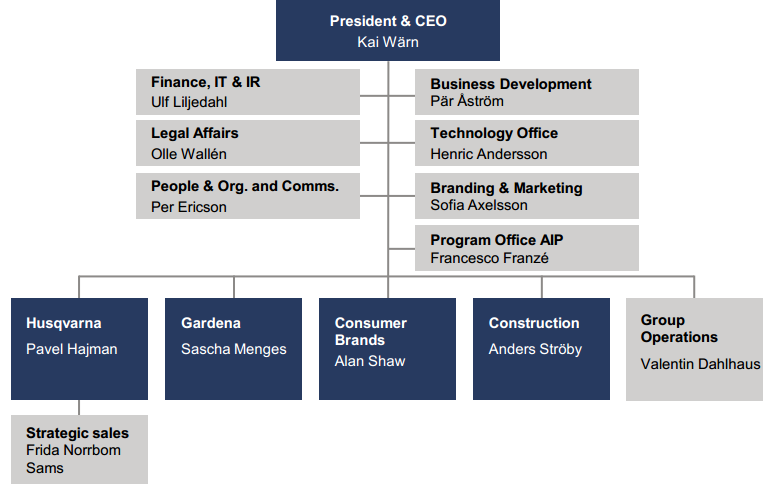
\includegraphics[width=0.9\textwidth]{img/organograma.png}
%	\caption{Organograma da empresa}
%	\label{organograma}
%\end{figure}

\subsection{Instalações}
	
	Na Alemanha a empresa não possui plantas de produção, porém existem dois depósitos e um escritório de vendas. O escritório - responsável por toda a Alemanha - e um dos depósitos estão localizados na cidade de Niederstotzingen, em Baden-Wurtemberg, à cerca de 100 km de Stuttgart. O segundo depósito fica na cidade de Müllheim, próximo à fronteira com a França.

	Diante da ausência de planta de produção no país, o número de funcionários na Alemanha é baixo. São menos de 50, que fazem todas as atividades de vendas, despacho, compras e afins. Na figura \ref{fig:organograma} pode-se ver a estrutura administrativa da Husqvarna e do escritório de vendas na Alemanha.

\begin{figure}[h!]
	\centering
	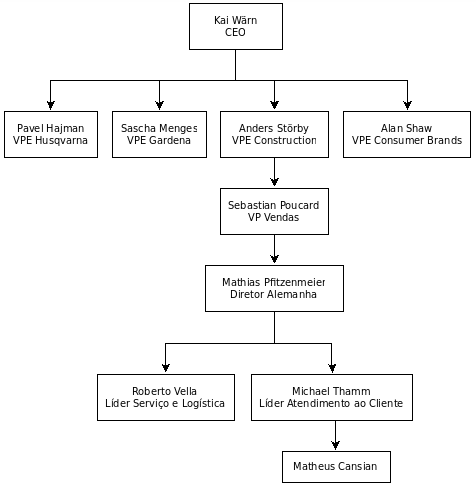
\includegraphics[width=0.9\textwidth]{img/organograma-matheus.png}
	\caption{Organograma Husqvarna}
	\label{fig:organograma}
\end{figure}

\clearpage

\section{Conceitos de administração financeira}

\subsection{Preço, Custo e Valor}
	
	Existem alguns conceitos financeiros envolvidos em operações de venda que são importantes de se compreender, porém são normalmente confundidos entre si. São eles:

\subsubsection{Preço}

	Preço é a quantidade de pagamento ou compensação dado por uma parte à outra em troca de produtos ou serviços. Na economia moderna, o preço é normalmente expressado em relação a uma moeda corrente. Juntamente com a definição de preço existe outra conhecida como Preço de Venda. Este nada mais é que o valor que uma parte pede à outra em troca de mercadorias ou serviços. O Preço de Venda pode ser diferente do Preço da Transação se, por exemplo, o vendedor der algum desconto.

\subsubsection{Custo}

	Custo corresponde à quantidade de dinheiro utilizado para produzir algo. Os custos podem ser divididos em fixos e variáveis. Custos variáveis são todos aqueles que estão diretamente ligados à produção de algo. Quanto maior a quantidade de itens produzidos, maior o custo variável. Por outro lado, os custos fixos são custos necessários para a produção de algo, mas que não variam com a quantidade de itens produzidos. Um exemplo de custo fixo é o aluguel de um galpão de fábrica.

\subsubsection{Valor}

	O valor é, muitas vezes, confundido com o preço, pois normalmente é expressado em unidade de moeda corrente, porém trata-se de um conceito econômico que é definido por alguns fatores como: usabilidade intrínseca ao produto, a demanda que o mercado tem por este produto, bem como a sua oferta. É possível resumir o conceito de valor respondendo à seguinte pergunta: "Qual é o preço máximo que um cliente pagaria por este produto?".

	Dentro do marketing existe um outro conceito chamado de Valor Percebido. Ele é, basicamente, a divisão entre o Valor de um produto e o seu Preço. O Valor Percebido é o que rege a ação de compra de um determinado consumidor. Quanto maior for o valor percebido, mais provável é que o consumidor efetue a compra de um produto ou serviço. Vale lembrar que o Valor Percebido não é simplesmente o valor econômico, mas sim algo mais subjetivo, que leva em conta questões como popularidade, grife, sazonalidade, etc.

	Um exemplo simples da subjetividade do Valor é um pacote de café brasileiro vendido no Brasil e na Europa. Os clientes europeus veem um valor maior no produto (por ter vindo do Brasil) do que os clientes brasileiros. Se o pacote de café fosse europeu, essa relação de valor provavelmente se inverteria.

\subsection{Finanças Corporativas}

	Para uma empresa, o indicador mais confiável do seu sucesso presente é o lucro líquido. No entanto, existem muitos outros indicadores intermediários que também são muito importantes. Todos esses indicadores possuem uma regra geral definida academicamente, entretanto a sua aplicação no dia-a-dia da empresa nem sempre segue a regra à risca. Na maior parte dos casos, algumas simplificações são realizadas. O objetivo delas é a economia de tempo, com perda pouco significativa no resultado final.

\begin{figure}[h!]
	\centering
	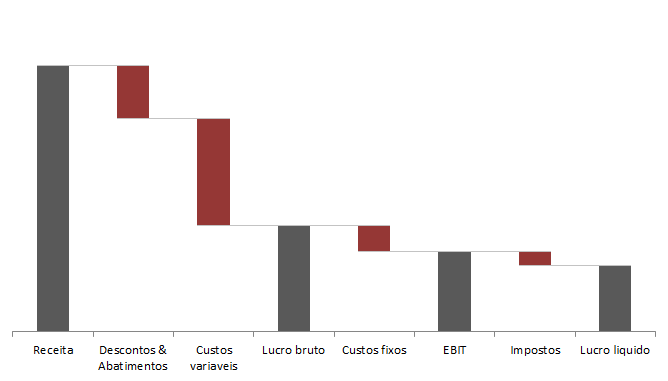
\includegraphics[width=0.9\textwidth]{img/finance.png}
	\caption{Representação esquemática do calculo de lucro líquido}
	\label{fig:lucro}
\end{figure}

	A figura \ref{fig:lucro} mostra uma das representações mais simples utilizadas para o cálculo do lucro líquido através de deduções da receita obtida pela empresa. Nos itens abaixo serão discutidos alguns dos indicadores intermediários, seus cálculos e utilização. 

\subsubsection{Receita}

	Receita é a entrada monetária que ocorre dentro de uma empresa, normalmente relativa às vendas de mercadorias ou serviços. As receitas podem ser brutas ou líquidas e operacionais ou não-operacionais. A receita bruta é aquela que corresponde ao valor negociado na aquisição de um produto e é a utilizada para cálculo de impostos sobre as vendas. A receita líquida então é a receita bruta descontada de devoluções, impostos diretos sobre o valor de venda e abatimentos.
A receita operacional é toda aquela proveniente da atividade principal de uma empresa, enquanto a receita não-operacional é resultado de atividades não principais da empresa. Um exemplo de receita não-operacional são aplicações financeiras.

\subsubsection{Desconto e Abatimento}

	Desconto e abatimento são reduções no preço de um produto realizadas para determinados clientes ou grupo de clientes. A diferença básica entre desconto e abatimento é que o primeiro refere-se a uma redução realizada antes da emissão da nota fiscal, enquanto o segundo é realizado depois. Comumente os descontos são utilizados por empresas para incentivar um cliente a comprar determinado produto ou a não comprar um produto similar do concorrente. Abatimentos são utilizados para incentivar um cliente a comprar quantidades maiores de determinados produtos. As compras podem ser realizadas em datas diferentes e o cliente recebe um abatimento no valor da compra quando atinge determinada meta de volume.

\subsubsection{Custos Variáveis}

	Custos variáveis são todos aqueles que têm relação direta com a quantidade produzida. Para uma indústria, os custos variáveis podem ser: matéria prima, mão de obra direta, energia elétrica direta, entre outros. Para o caso de um escritório de vendas, os custos variáveis são o preço interno e o custo de transporte da fábrica até o depósito.

\subsubsection{Lucro Bruto}

	Lucro Bruto corresponde à receita líquida menos os custo variáveis. Ele revela o quanto o produto gera de lucro, sem levar em consideração a estrutura administrativa e seus respectivos custos fixos.

\subsubsection{Custos Fixos}

	Custos fixos são todos os que não são proporcionais ao volume produzido. Isto inclui o salário do setor administrativo, aluguel, energia utilizada em atividades não produtivas, etc.

\subsubsection{EBIT}

	EBIT é a sigla em inglês para Earnings Before Interest and Taxes (Lucro antes de Juros e Imposto de Renda). Ele é correspondente ao lucro total obtido pela a empresa sem levar em conta a política de distribuição de lucros, juros de empréstimos anteriores, bem como impostos sobre o lucro. O EBIT tem duas finalidades: a primeira é enquanto indicador de como a empresa esta performando no presente - como este valor não leva em conta o pagamento de juros, o lucro da empresa do período não é punido por empréstimos que a empresa fez no passado; a segunda função é ter uma relação entre duas empresas distintas - como o EBIT desconsidera o pagamento de impostos, ele não está punindo uma empresa que encontra-se em um país no qual os impostos são maiores. O EBIT também não considera a distribuição de lucros, ou seja, não pune uma empresa que distribui mais lucros para os seus acionistas.

\subsubsection{Impostos}

	Impostos são a última dedução realizada antes do lucro líquido. O imposto deduzido nesta etapa corresponde ao imposto sobre o lucro obtido.

\subsubsection{Lucro Líquido}

	Lucro líquido é o capital que sobra para a empresa após cumprir todas as suas obrigações fiscais e legais.

\subsection{Efeitos Financeiros}

	Efeitos financeiros são os impactos que ocasionam uma diferença financeira entre dois períodos. A maior utilização desse conceito é para verificação de quais podem ter sido as causas que trouxeram uma diferença de lucro, rentabilidade ou custo num determinado período. Não existe classificação fixa para quais são os efeitos financeiros. Por regra, os mais utilizados para o cálculo de diferença de lucro são: Volume, Preço, Custo e Mix.

\begin{figure}[h!]
	\centering
	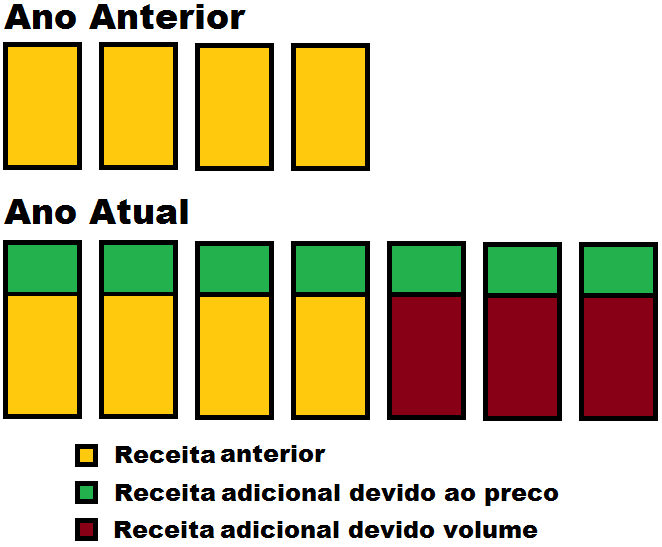
\includegraphics[width=0.6\textwidth]{img/effects.png}
	\caption{Representação esquemática dos efeitos de volume e preço}
	\label{fig:effects}
\end{figure}

	Na figura \ref{fig:effects} pode-se ver uma representação simples dos efeitos de volume e preço na rentabilidade entre dois anos. Cada retângulo corresponde a um produto vendido e a sua área a rentabilidade total. No primeiro ano foram vendidos quatro produtos. No ano seguinte, foram vendidos sete produtos, com leve aumento de preço. A área em amarelo corresponde ao faturamento referente ao ano anterior; em verde, devido ao aumento de preço e em vermelho, devido ao aumento de volume.

%\subsubsection{Efeito Volume}
%Corresponde ao lucro adicional, ocasionado pelo aumento de volume de vendas.
%\subsubsection{Efeito Preco}
%\subsubsection{Efeito Custo}
%\subsubsection{Efeito Mix}

\section{Projetos Realizados}

	O estágio foi realizado no escritório de vendas da Alemanha, sendo as principais atribuições do estagiário o desenvolvimento de projetos para aumentar indicadores de vendas e a prestação de apoio nas atividades do dia-a-dia. Durante o período, dois projetos foram de grande importância e ajudaram a desenvolver áreas da empresa que estavam aquém de seu potencial. O primeiro deles trata-se de uma nova metodologia para precificação de peças de reposição, enquanto o segundo foi direcionado ao desenvolvimento de um programa de manutenção para um dos produtos fabricados pela Husqvarna. Devido ao tempo de duração do estágio, o segundo projeto limitou-se a apenas uma máquina, mas o modelo de negócio escolhido pode ser utilizado para os demais produtos.

\subsection{Política de precificação para peças de reposição}

	Os equipamentos da Husqvarna para a construção civil são focados no público profissional. Isto significa que as máquinas devem ser desenvolvidas para uma alto número de horas de uso. Por este motivo, falhas são frequentes e a disponibilidade e preço das peças de reposição são dois dos principais motivadores que fazem as empresas comprar os produtos do Grupo. O objetivo deste projeto foi analisar a precificação que a Husqvarna faz para as peças de reposição em comparação aos seus concorrentes, bem como a maneira como o cliente avalia o valor de uma peça. A partir disto, foi montada uma estratégia de preços, visando o aumento do faturamento da empresa e da satisfação do cliente.

	Na maioria da empresas, a conta que se realiza para o cálculo de preço é, basicamente, utilizar o custo de determinado produto e adicionar uma margem esperada. O problema desta abordagem é que, não levando em conta o preço do mercado, pode-se estar vendendo mais caro do que o cliente esperava pagar (perdendo assim volume) ou vendendo mais barato do que o cliente pagaria (perdendo assim lucro). A maneira ideal de se obter o preço de um produto é fazer a análise inversa: Qual é o preço máximo que o meu cliente estaria disposto a pagar por este produto? Através da resposta à esta questão, é possível descontar do preço uma margem interessante de lucro para a empresa e com isso, estabelecer o custo máximo viável para que o produto seja considerado rentável.

	A Husqvarna, por ser uma empresa global, tem uma dificuldade especial: a diferença de preços entre países. A Europa é um continente no qual os laços comerciais entre os países são muito fortes e é fácil para uma empresa analisar o preço de determinado produto no exterior. Diante disso, os preços da Husqvarna devem fazer sentido não só para a Alemanha, mas devem estar alinhados com o que os outros países cobram (França, Países Baixos, Áustria, etc). Via de regra, os preços em determinado país poder ser mais altos, mas isto aplica-se a todo o portfólio de produtos e não apenas a um produto, isoladamente.

	Outro fator importante nessa análise é o fato de que muitos clientes heavy users possuem várias máquinas diferentes. Isto permite que eles façam comparações entre máquinas. Um exemplo disto seria um cliente que possui uma serra grande e uma pequena: ele pode comparar os preços das peças de reposição e aceitar que o filtro de ar para uma máquina grande é mais caro que um para máquina pequena, porém julgar que o contrário não é coerente. Neste caso, o cliente pode entender que o filtro para a máquina pequena está muito caro.

	O primeiro passo deste projeto foi levantar estes problemas e realizar um Brainstorming de soluções. Sendo a Husqvarna uma empresa grande, o problema torna-se de difícil resolução e é esperado que nem todos os pontos para todos os produtos possam ser completamente solucionados. A ideia do projeto, entretanto, é ao menos amenizar essas dificuldades.

\begin{figure}[h!]
	\centering
	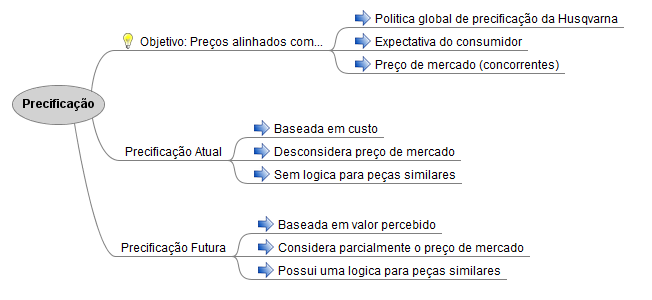
\includegraphics[width=0.9\textwidth]{img/pricing-pt.png}
	\caption{Objetivos do projeto de precificação}
	\label{fig:pricing}
\end{figure}

	Historicamente, os preços das peças de reposição eram calculados com base no custo. As margens de cada filial eram previamente definidas e somando-as ao custo, obtinha-se o preço final. O principal ponto de atenção deste método é que ele não leva em conta o preço de mercado. Simplesmente adicionando uma margem ao custo, não existe qualquer garantia de que o produto vendido tem preço competitivo. Além do exposto, esta visão não contribui para a redução de custos da empresa, tendo em vista que ela não proporciona a definição de qual custo alvo deve ser buscado.

\subsubsection{Indicador de valor}

	O primeiro passo para corrigir este problema foi trabalhar em conjunto com a matriz, obtendo preços de outros países para cada produto. Como primeiro balizador, obteve-se a média internacional de preços para cada produto. Observando estes números, notou-se que eles apresentavam algumas divergências.

	É conhecido que o custo de fabricação de um produto depende muito da quantidade produzida. Quanto maior a quantidade, menor o custo. O fato é que as máquinas mais vendidas pela Husqvarna são as máquinas menores (pois atendem tanto ao público de uso doméstico quanto o profissional) e por isso o custo de suas respectivas peças de reposição são menores do que as de máquinas maiores. Para o cliente final, a estratégia de produção da Husqvarna, ou o seu portfólio de clientes, não tem nenhuma relação com a decisão de compra. O cliente utiliza mecanismos mentais simples para tomar essas decisões. Por exemplo, para o cliente, um motor de uma máquina menor deve ser necessariamente mais barato do que o de uma máquina maior. Entretanto, devido a produção da Husqvarna, nem sempre isso acontece.

	Para contornar essa visão do cliente, novos critérios tiveram que ser definidos para o cálculo do preço. Foi criado um índice chamado de "indicador de valor" que é, basicamente, o parâmetro que o cliente enxerga no produto como valor. No caso de um motor por exemplo, utilizou-se a cilindrada. Quanto maior a cilindrada, maior o preço. No caso de parafusos, foi o peso. Quanto mais pesado e aparentemente robusto um parafuso, mais ele custa. A tabela \ref{tab:valor} mostra o indicador de valor utilizado para alguns grupos de peças.

\begin{table}[!h]
	\centering
	\caption{Exemplos de indicador de valor}
	\begin{tabular}{| l | l |}
		\hline
		Produto & Indicador de valor \\ \hline
		Filtro de ar & Potência do motor \\
		Motor & Cilindrada \\
		Parafuso & Peso \\
		\hline
	\end{tabular}
	\label{tab:valor}
\end{table}

\subsubsection{Preço de mercado}

	Através do indicador de valor, foi possível melhorar a análise de preço. Os preços que antes eram baseados apenas em custo, agora não dependem mais da estratégia de produção da Husqvarna e fazem mais sentido para o cliente final. No entanto, isso não foi suficiente. Para que fosse obtido preço ainda melhor, foi necessário descobrir qual era o preço de mercado de cada produto.

	O preço de mercado corresponde a uma média de preços realizada por todos as empresas dentro de um mercado específico. Com o objetivo de obter essa informação, realizou-se uma pesquisa de mercado através da obtenção de lista de preços de revendedores multi-marcas, pedidos de cotação enviados para revendedores de concorrentes e através da análise do time de vendas. Utilizando os dados coletados, foi realizado ajuste dos preços já calculados. Na figura \ref{fig:competitor} pode-se visualizar o preço médio internacional de um cilindro de motor após a aplicação do "indicador de valor" (linha azul fina); o preço na Alemanha após o "indicador de valor" (linha azul grossa); os preços de mercado obtidos através de pesquisa (pontos); e o preço calculado após os dados de mercado (linha roxa). O eixo horizontal corresponde as cilindradas do motor que é o seu indicador de valor.

\begin{figure}[h!]
	\centering
	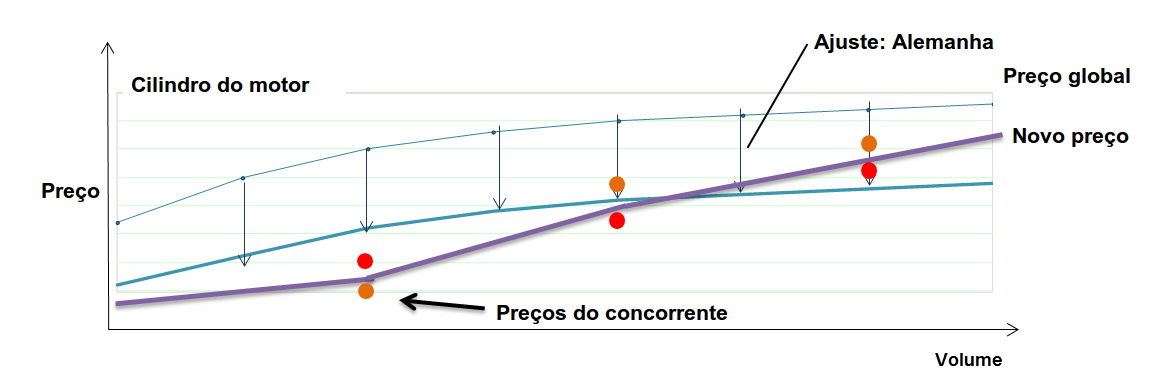
\includegraphics[width=0.9\textwidth]{img/wettbewerber-pt.png}
	\caption{Cálculo de preço com base no indicador de valor}
	\label{fig:competitor}
\end{figure}

\subsubsection{Movimentação de preços}

	Apenas o cálculo dos preços não é o suficiente, pois outro fator importante sobre precificação é que ela não pode ser realizada em movimentos bruscos. O aumento muito acentuado de preços pode fazer com que os consumidores troquem de fornecedor, mesmo que os preços estejam agora em patamares justos. Da mesma forma, uma redução drástica, sem nenhuma campanha de marketing, gera um impacto negativo na margem de lucro e quase nenhum aumento no volume de vendas. Para contornar o problema foram definidos algumas categorias de produtos e para cada uma, cenários de mudança de preço.

	A primeira categoria são os "preços errados". Foram detectados alguns preços que estavam significativamente desconexos da realidade de mercado. Algumas peças possuíam um valor muito aquém ou além do seu preço alvo, provavelmente resultantes de erros de digitação ou de análises realizadas no passado. Para esses produtos a solução é direta. Todas as peças tiveram o seu preço modificado para o preço alvo, independente do tamanho da alteração.

	Uma particularidade de precificação vem do termo "transparência de mercado", que representa o quanto o cliente sabe sobre o preço de mercado de determinado produto. Dentro dessa teoria, o cliente só tem como saber se algo é caro ou barato se tiver alguma outra referência para calcular. Utilizando-se disto, criou-se uma segunda categoria. Esta categoria contém as peças antigas que não obtiveram nenhuma venda desde 2011. Isto corresponde à reposição de máquinas antigas que estão, aos poucos, saindo do mercado. Como o cliente não tem a possibilidade de realizar a comparação histórica de preços, ficou definido que todos seriam modificados diretamente para o alvo.

	Na terceira categoria enquadraram-se as peças de pouco valor agregado. Estas são peças com preço inferior a 10 euros e correspondem a parafusos, pequenas juntas mecânicas, gaxetas, etc. Como o seu valor monetário é baixo, mudanças grandes em porcentagem, se convertem em pequenos valores em euros. Um exemplo disso é uma peça com um preço de 2 euros. Um aumento de 30\% corresponde apenas a um adicional de 60 centavos. Para essas peças foi definida a mudança direta para o preço alvo, quando ele também for inferior a 10 euros.

	Por último, para todas as outras peças, foi definido um cenário onde a mudança máxima de preço é 3\%. Esse valor foi calculado para se aproximar da média de aumento anual de preços da Husqvarna. Fazendo a análise de todas as mudanças de preço o aumento médio ponderado foi igual a todos os outros anos. Isto garante que o aumento da margem de lucro será equivalente ao histórico, só que desta vez, com os preços mais bem calculados, o aumento de volume é muito provável.

\subsection{Serviço de manutenção de serras de parede}

\begin{figure}[!ht]
	\centering
	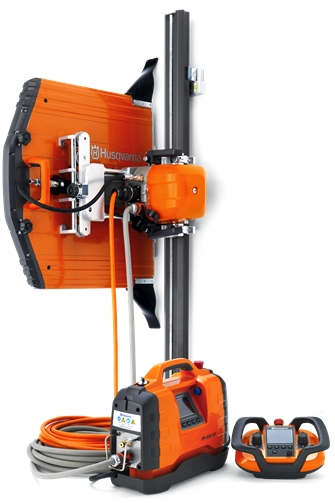
\includegraphics[width=0.4\textwidth]{img/ws220_produto.png}
	\caption{Serra de parede modelo WS220}
	\label{fig:ws220_produto}
\end{figure}

	Para um empresa prestadora de serviços de construção na Alemanha, os gastos referentes à aquisição e manutenção das ferramentas de trabalho correspondem a um valor expressivo do custo total da empresa. Além disso, o ambiente agressivo e o uso constante ao qual as máquinas são expostas são motivos frequentes de falhas, até mesmo nas máquinas mais robustas. Para um empresa menor, que possui poucas máquinas, a falha de uma delas pode ter consequências devastadoras na prestação de serviços. Além dos custos de reparo, os dias em que a empresa fica impossibilitada de trabalhar gera grande impacto negativo no fluxo de caixa.

	O objetivo do projeto foi desenvolver um pacote de manutenção para transferir o risco de fluxo de caixa do cliente para a Husqvarna. Uma venda suficientemente grande de pacotes de manutenção é para a Husqvarna uma boa maneira de mitigar o risco de fluxo de caixa, tendo em vista que apesar das falhas serem imprevisíveis, é possível que a empresa calcule uma média de gastos anuais. Com um número suficientemente grande de máquinas, a probabilidade de as falhas ocorrerem em um mesmo mês é extremamente baixa. Para esse projeto específico, foi escolhida uma serra de parede modelo WS220 (figura \ref{fig:ws220_produto}). O motivo da escolhe deve-se ao fato que esse modelo é lançamento no mercado e por isso é mais fácil apresentar a novidade aos clientes.

	Utilizando a metodologia do Balance Scorecards (BSC), o projeto foi divido em etapas, cada uma correspondendo a um fator crítico de sucesso. Os fatores do BSC podem ser visualizados na figura \ref{fig:bsc}. 
	
	Para o quesito Financeiro foi definida a realização de uma análise de custos do produto; para o fator Cliente, foi realizada análise na questão de precificação do produto e serviços; na questão de Processos Internos foi desenvolvida toda a documentação relacionada ao pacote, de forma que a aplicação desse projeto fosse realizada de forma fácil e sem erros por parte da empresa; por último, na questão Aprendizagem e Crescimento, foi criada documentação do projeto visando que a replicação para outros produtos fosse relativamente fácil. Na figura \ref{fig:service} pode-se ver uma análise geral das questões a serem respondidas pelo projeto.

\begin{figure}[h!]
	\centering
	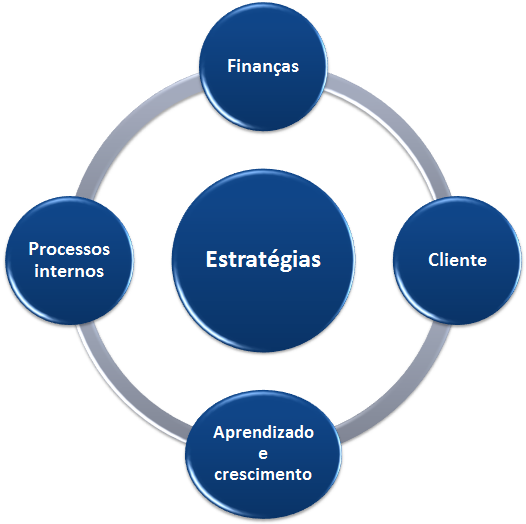
\includegraphics[width=0.4\textwidth]{img/bsc.png}
	\caption{Matriz BSC}
	\label{fig:bsc}
\end{figure}

\begin{figure}[h!]
	\centering
	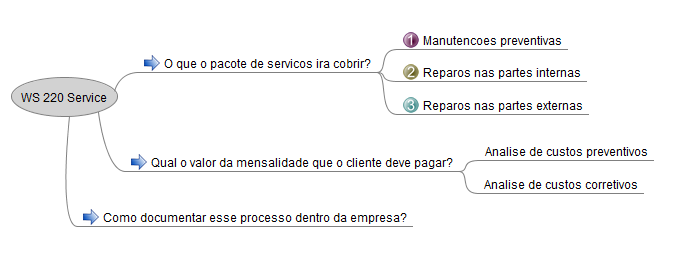
\includegraphics[width=0.9\textwidth]{img/ws220.png}
	\caption{Objetivos do projeto de serviço}
	\label{fig:service}
\end{figure}

\subsubsection{Análise de custos e precificação}

	Para o custo de manutenção preventiva, utilizou-se o manual de reparos do produto para efetuar lista de serviços de manutenção que devem ser realizados a cada intervalo de tempo. Com base nesses dados, foi calculado o custo desses serviços com base no preço interno. Além disso, o custo da mão-de-obra foi determinado pelo time de manutenção. Com base nos serviços que devem ser realizados, o time deu uma estimativa de horas para completar. Com base nessa estimativa e no custo de uma hora de trabalho foi estimado o custo de mão-de-obra.

\begin{figure}[h!]
	\centering
	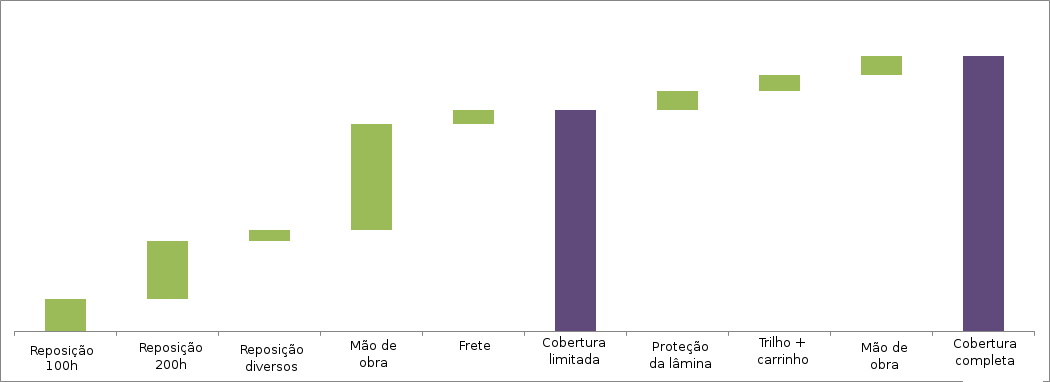
\includegraphics[width=0.9\textwidth]{img/ws220-waterfall-pt.png}
	\caption{Cálculo de custos do projeto}
	\label{fig:ws-waterfall}
\end{figure}

	Em relação à análise de custos, primeiramente foram obtidos os dados sobre taxas de falhas para cada componente da máquina. Esses dados correspondem à média de produtos que apresentam falha a cada 100 horas de uso. Esses dados foram então calculados para um cenário de mil produtos e 500 horas de uso. Os resultados obtidos correspondem às peças que a empresa deveria repor na vida útil de mil máquinas. 
	
	A partir da lista de peças, o custo total de reposição foi calculado utilizando como base no preço interno + frete. Esse custo corresponde ao de manutenção corretiva, pois representa apenas a substituição de componentes após eles apresentarem falha. A mão de obra foi calculada utilizando o custo das peças e a estimativa da manutenção preventiva. Na figura \ref{fig:ws-waterfall} pode-se visualizar os dados finais da análise de custo (os valores foram removidos do gráfico por serem dados confidenciais). O custo total de manutenção é a soma dos custos de manutenção preventiva, corretiva e transporte da máquina. Com base nesse custo foi possível adicionar a margem de lucro da empresa e obter o preço final para o cliente.
	
\subsubsection{Documentação externa e interna}

	Seguindo a análise do BSC para os quesitos de Processos Internos e Aprendizagem e Crescimento, foram desenvolvidas documentações externas e internas. Para atender essa demanda, foram produzidos 4 documentos diferentes: Contrato; Caderno de Serviço; Protocolo de Entrega e Manual Interno.

	Para o contrato, utilizou-se o modelo padrão da Husqvarna, onde a definição das cláusulas fizeram parte do escopo do projeto. O caderno de serviços é um folheto no qual o usuário tem as informações sobre a sua máquina, os planos de manutenção e um espaço em que o técnico de manutenção pode carimbar a cada serviço feito. O protocolo de entrega constitui em um contrato assegurando que o cliente recebeu todas as partes da máquina e suas devidas instruções e, por último, o manual interno contém os processo que devem ser seguidos dentro da empresa relacionados à esse projeto.

\pagebreak

\section{Observações referentes às informações do relatório
}
	Informações como dados financeiros, estratégias de marketing e dados sobre produtos são consideradas sigilosas e portanto, foram omitidas neste relatório, respeitando a política de confidencialidade da Husqvarna.
\pagebreak

\section{Considerações finais}
	
	Embora o trabalho na área de vendas envolva muitas questões humanas, como relacionamento com clientes, os aspectos exatos tem uma grande parcela de importância. Antes da comunicação com o cliente é importante definir a estratégia que o time de vendas deve seguir, os preços, os serviços e diversos outros fatores. Para a maior parte dessas atividades, habilidades em raciocínio lógico e matemática, características fundamentais de um engenheiro, são os principais requisitos para a realização de um trabalho de qualidade. Ademais, nem sempre a decisão de compra de um cliente é baseada em racionalidade e exatidão. Isso cria um desafio adicional para o engenheiro que está acostumado a equações e resultados exatos. A solução para isso deve ser buscada junto à literatura, na qual se encontra alguns conceitos de administração que auxiliam na determinação dos fatores emocionais dos clientes.
	
	A área de vendas apresenta alguns desafios que não são encontrados, por exemplo, na área de projetos. Entretanto, o perfil de engenharia, aliado com o estudo de alguns conceitos de administração torna esse profissional extremamente qualificado para a entrega de resultados.
\pagebreak

\section{Referências}
	{
		\noindent
		Balanced Scorecard. Disponível em: <wirtschaftslexikon.gabler.de/Definition/balanced-scorecard.html>. Acesso em: 16 de novembro de 2014. \\
		\\
		História da Husqvarna. Disponível em: <www.husqvarna.com/br/construction/company/history/>. Acesso em: 16 de novembro de 2014. \\
	}
\pagebreak

\end{document}
